\documentclass[journal]{IEEEtran}

\usepackage{blindtext}
\usepackage{cite}
\usepackage{graphicx}
\usepackage{array}
\usepackage{color}
\usepackage{tabularx}
\usepackage{epsfig}
\usepackage{amsmath}
\usepackage{amssymb}
\usepackage{bm}
\usepackage{wasysym}
\usepackage{circuitikz}
\usepackage{float}
\usetikzlibrary{arrows,shapes,calc,positioning}

\newcommand{\myscope}[2]
{\draw[thick,rotate=#2] (#1) circle (12pt)
(#1) ++(-0.35,-0.1) --++ (0.3,0.3) --++ (0,-0.3) --++(0.3,0.3) --++(0,-0.3);}

\begin{document}

\title{CSCE 221 \\ Problem Set 9}

\author{Jacob~Purcell,~\IEEEmember{Texas~A\&M,~Student}}

\maketitle
\section{}

A binary tree is defined such that each parent node has no more than 2 children. 
Let us consider the case of only one node($N_r$) with 2 children, the total
number of nodes is given by $N_r + 2 = 3 nodes$ with a height of 1. At height 2,
the expression becomes $N_r(h = 0) + 2(h = 1) + 2*2(h = 2)$ which leads to 

\begin{equation}
\Sigma_{h=0}^H 2^h
\end{equation}

Finding the closed form for this summation from the geometric series,

\begin{equation}
\Sigma_{n=1}^N ar^n = a(1 + r + r^2 \cdot \cdot \cdot r^N) = S
\end{equation}

Using the property that $1 + r + r^2 \cdot \cdot \cdot r^N = \frac{r^n - 1}{r - 1}$,

\begin{equation}
S = a \frac{r^n - 1}{r - 1}
\end{equation}

Finally, substituting known values established in $eq. 1$ into $eq. 3$, 
r = 2, n = h + 1, a = 1 leads to

\begin{equation}
S = 1 \cdot \frac{2^{h+1}-1}{2-1}
\end{equation}

\begin{equation}
\boxed{S = 2^{h+1} - 1}
\end{equation}

\section{}

Prefix, infix, and postfix notations are expressed as

\begin{equation}
    Prefix~:~[operator][operand][operand]
\end{equation}

\begin{equation}
    Infix~:~[operand][operator][operand]
\end{equation}

\begin{equation}
    Postfix~:~[operand][operand][operator]
\end{equation}

Using PEMDAS and starting from the bottom of the tree to connect the order of 
operands, the expression will begin as 

\begin{equation}
    \{(a+b)*c\} - \{d+e\}
\end{equation}

Using the predefined notations as a map, the expression becomes

\begin{equation}
    \begin{split}
    Prefix~:~-\{*(+ab)c\}\{+de\} \\
    -\{*+abc\}\{+de\} \\
    \boxed{-*+abc+de}
    \end{split}
\end{equation}

\begin{equation}
    Infix~:~\boxed{\{(a+b)*c\} - \{d+e\}}
\end{equation}

\begin{equation}
    \begin{split}
    Postfix~:~\{(ab+)c*\}\{de+\}- \\
    \{ab+c*\}\{de+\}- \\
    \boxed{ab+c*de+-}
    \end{split}
\end{equation}

\section{}

Insertion into a binary tree follows the pattern left < parent, while right > parent.  
Following this pattern and starting with 7, Fig. 1 shows the result of loading a binary
tree with the given sequence of numbers.

\begin{figure}[h!]
	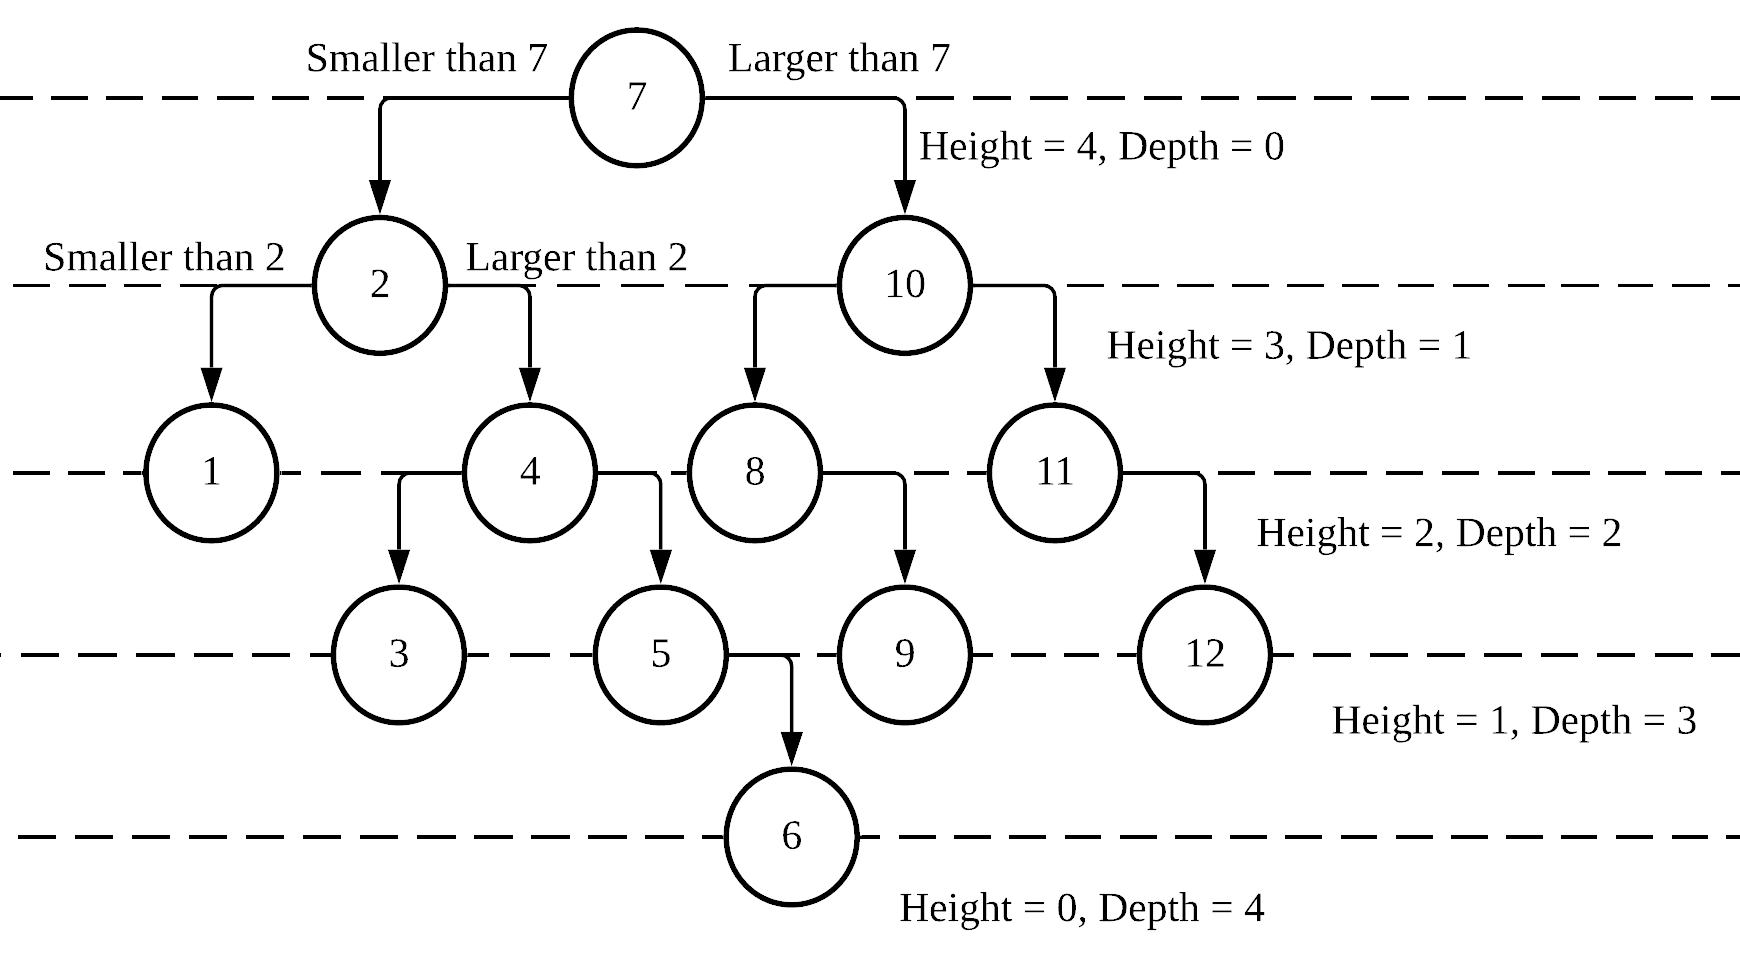
\includegraphics[scale = 0.13]{bt.png}
	\caption{Each dotted line represents a layer of the tree. \\ Each node in a layer shares the same height and depth.
             \\ Arrows point to left and right children.}
\end{figure}

\subsection{}

\subsubsection*{I}
7 is the head node. Since 7 is inserted into an empty tree, it is the only node and all 
other nodes will be its children.

\subsubsection*{II}
The leaves are 1, 3, 5, 6, 9, and 12 since the have no children.

\subsubsection*{III}
Siblings are child nodes that have the same parent. Since this is a binary tree, siblings come in pairs. Sibling pairs are

$$2 \& 10$$
$$1 \& 4$$
$$8 \& 11$$
$$3 \& 5$$

\subsubsection*{IIII}

Depth is measured from the top starting at 0, the nodes with corresponding depth are

$$0~:~7$$
$$1~:~2,~10$$
$$2~:~1,~4,~8,~11$$
$$3~:~3,~5,~9,~12$$
$$4~:~6$$

\subsubsection*{V}

Height is measured from the bottom starting at 0, the nodes with corresponding height are

$$0~:~6$$
$$1~:~3,~5,~9,~12$$
$$2~:~1,~4,~8,~11$$
$$3~:~2,~10$$
$$4~:~7$$


\subsection{}

Deleting the head node would require some restructuring to maintain tree integrity. 
We would need to replace it with the next largest value, so we traverse the 
left side of the right child to the end, then that node is deleted and takes 
the place of the root node.

\begin{figure}[h!]
	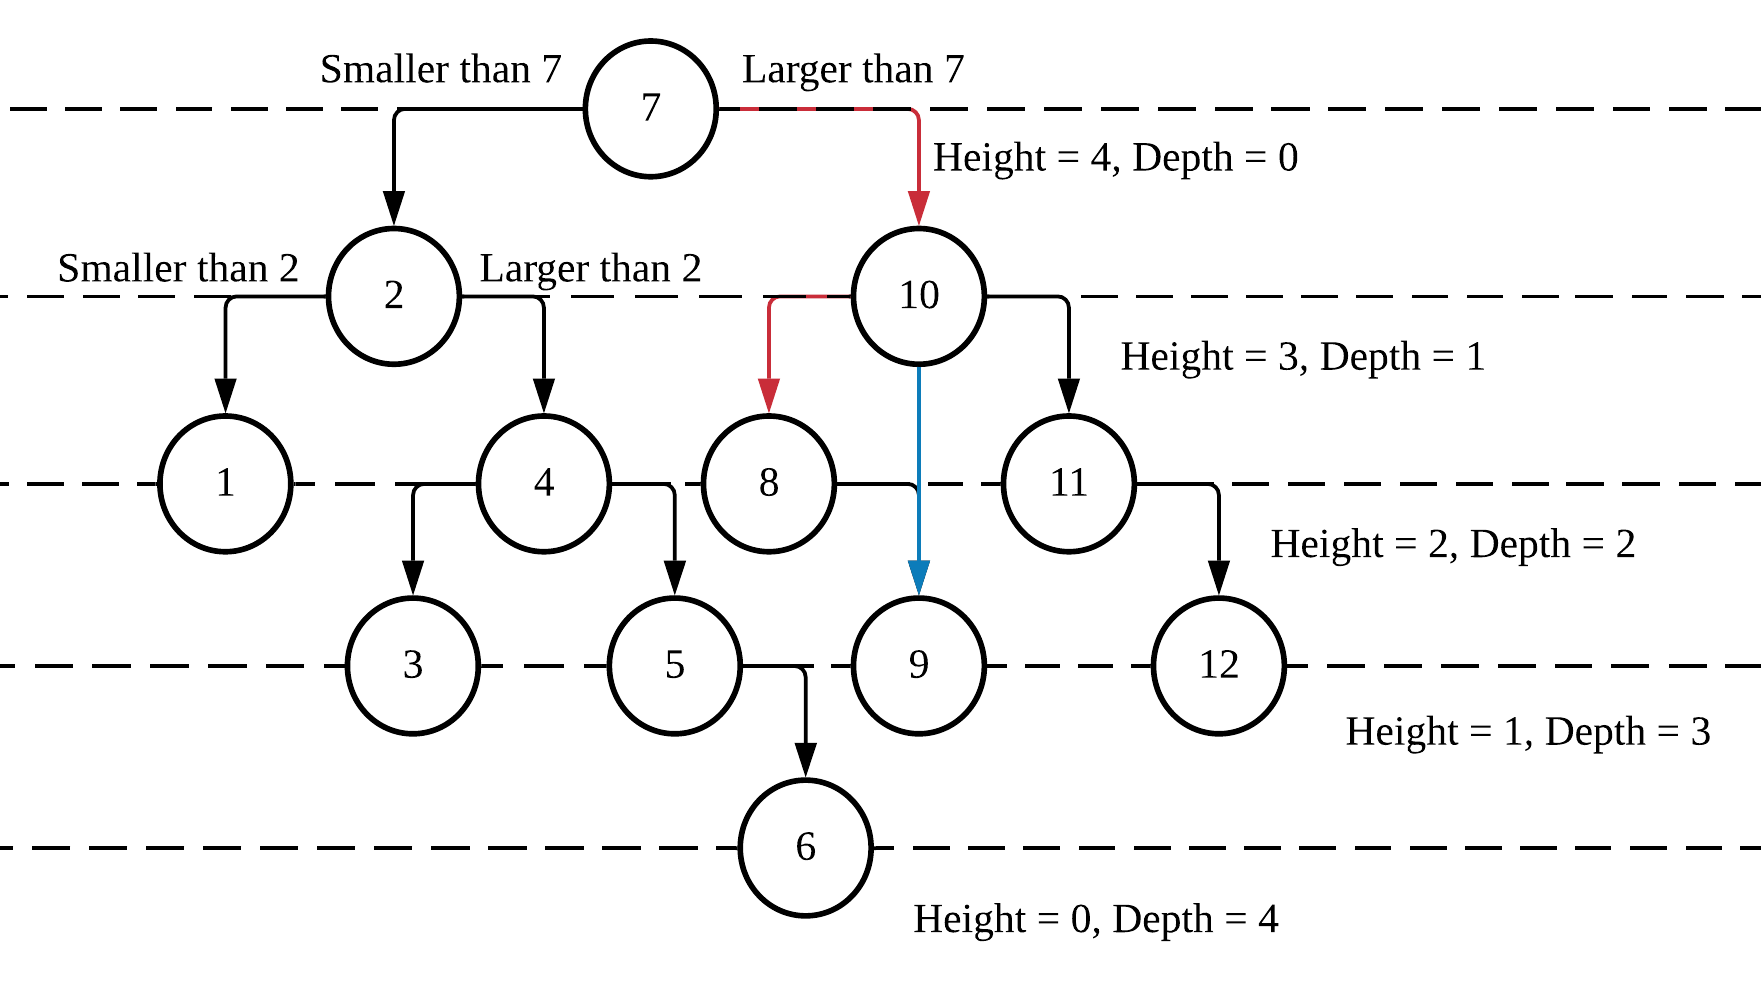
\includegraphics[scale = 0.13]{btp.png}
	\caption{Red shows the search path until the replacement node is found. \\ Blue shows the creation of a new left child path.}
\end{figure}
\begin{figure}[h!]
	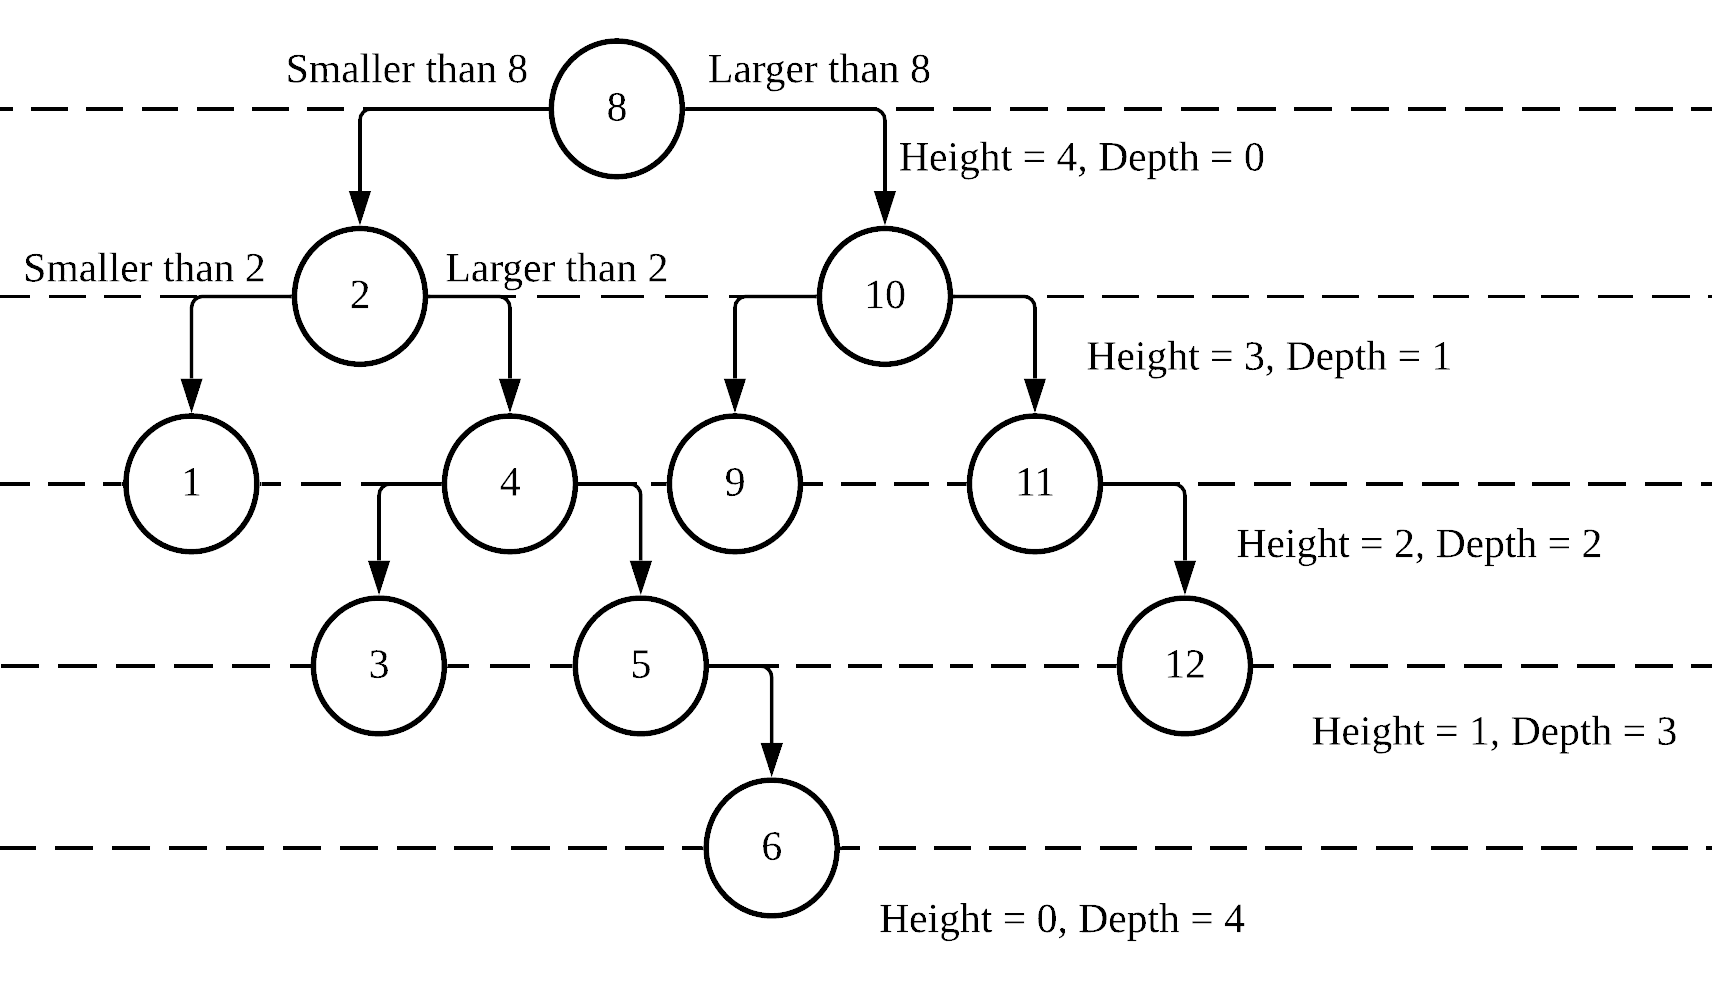
\includegraphics[scale = 0.13]{btr.png}
	\caption{The final result of deleting the head node.}
\end{figure}

\section{}

\subsection{}
    Included in "tree\_functions.h" lines 108-116. Return value 12 corresponds to Fig. 1.
\subsection{}
Included in "tree\_functions.h" lines 121-130. Return value 5 corresponds to Fig. 1.
\subsection{}
Included in "tree\_functions.h" lines 135-144. Return value 4 corresponds to Fig. 1.\\\\
"mainps9.cpp" is included as a demonstration where accuracy is confirmed. \\\\

Since every function accesses every node once, each function is $\boxed{O(N)}$ although they are defined using recursion.

\end{document}
